\documentclass[11pt]{article}
\usepackage{amssymb,amsmath,amsthm,url,subfigure, multirow,hyperref}
\usepackage{graphicx}
\usepackage{color}
\usepackage{enumerate}

\usepackage{gensymb}
\newcommand\eat[1]{}

\begin{document}
\eat{
\section{Plan}
At a high level the idea (was/is at this point/might be) is:
\begin{itemize}
\item Somehow get our hands on a model of all (most) middleboxes in the
network. This might be computed using program analysis or be provided by
someone etc.
\item Hook up middleboxes as a network, verify that some high level policies (for instance isolation) holds given the model. 
\item If step 2 reveals that things are peachy, generate some packets to verify that the model itself is actually behaving reasonably.
\item Prosper.
\end{itemize}

For now we (I) are focusing on step 2. In particular the plan is to generate models for a variety of middleboxes and
see what we could do with this. Since I was having a hard time actually doing the model generation (I did not know what
part of the model was relevant, amount of detail required, etc.), I decided to generate only two models and try and
actually prove something in a simple network.

For what follows, most of the proofs and such were generated using \href{http://z3.codeplex.com/}{Z3} a SMT solver from
MSR.

\section{Middleboxes so Far}
This is a list of middle boxes modeled so far:
\begin{itemize}
\item Packet Filters (simple ACL firewalls)
\item Stateful firewalls
\item Web proxies
\item Learning switches.
\end{itemize}

\section{Results so Far}
\begin{figure*}[!h]
\begin{center}
\subfigure[Firewall then Web Proxy]{
    \centering
    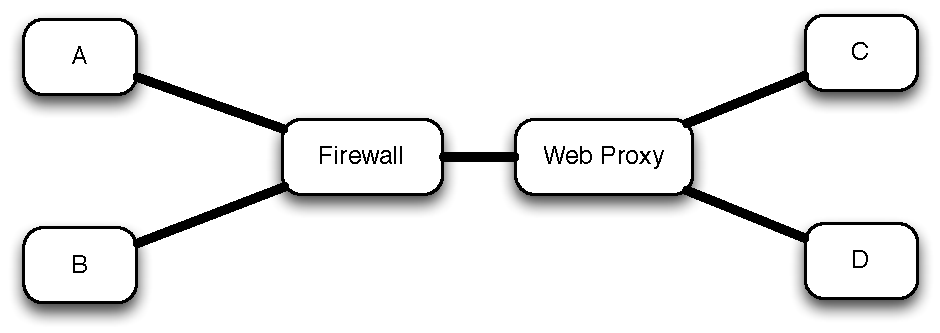
\includegraphics[width=0.47\textwidth]{./firewallwebproxy.pdf}
    \label{fig:fwwp}
}
\subfigure[Webproxy then Firewall]{
    \centering
    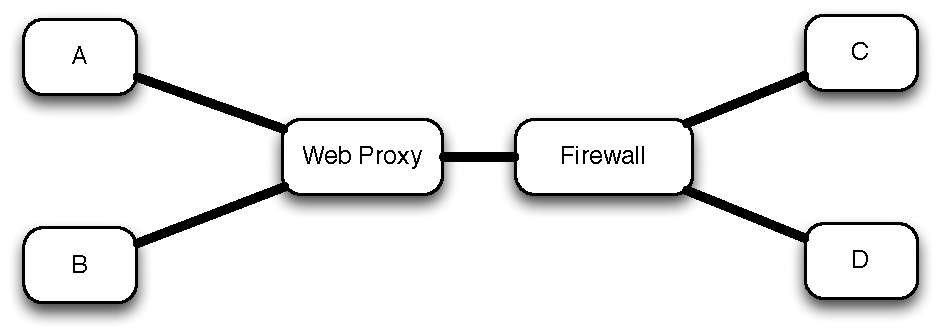
\includegraphics[width=0.47\textwidth]{./webproxyfirewall.pdf}
    \label{fig:wpfw}
}
\caption{Two topologies}
\label{fig:topologies}
\end{center}
\end{figure*}
Consider the two topologies in Figure~\ref{fig:topologies} and Firewall rules that disallow communication between
endhosts $A, C$ and $B, D$. Globally we want to ensure that $B$ cannot ever induce a packet to be sent to $D$ and $A$
cannot ever induce a packet to be sent to $C$. This policy is only enforceable in Figure~\ref{fig:fwwp} since the packet
looses information that is required for enforcement when it goes through the web proxy.

Currently we can generate counter examples for Figure~\ref{fig:wpfw} where the global policy does
not hold. Similarly for Figure~\ref{fig:fwwp} it can prove that the global policy does hold (by showing that no packets
satisfy the negation of the global constraints). 

We can also generate results with stateful firewalls for the same topologies, where depend on firewall rules even Figure
~\ref{fig:fwwp} can have a policy violation. Furthermore, we can even generate a counter example where the firewall is entirely 
correct but we model the response part of the web proxy. In reality the only way to ensure isolation in either of these
topologies is to either have firewalls on both sides of the proxy or model the end hosts as servers and clients, where servers
never generate any requests.

\section{Other Concerns}
First-order logic with quantifiers ($\forall$ and $\exists$) is
undecidable and will sometimes trip up the solver. Normally one tries to reexpress the constraints or add additional
(redundant) constraints for the solver to work, but I haven't yet figured out what combination of constraints will help.
This is generally a problem for this sort of thing, but on average proof that there is a bug can be gotten really
quickly, but proving that there is no bug can take quite long.

\section{What is New}
A few things are different now:
\begin{itemize}
\item We actually account for things like routing tables now, so hooking into something like HSA should be simpler.
\item Stateful middleboxes like learning firewalls (also learning switches, but at least for analyzing isolation they are
not super interesting).
\item A saner model (it is easier to analyze and figure out what is wrong).
\end{itemize}

\section{Next Steps}
Now that most of the modeling seems to work quite well there were a few different things I was considering doing next:
\begin{itemize}
\item Add support for time: currently we flatten out time in some sense, and this will become a problem as we start generating 
test since state changes depend on time. I think this should be simple.
\item Model end hosts more richly to state what they would generate requests for. I feel a bit fishy doing this but then again without making
    some assumptions about the behavior of everything we end up with models where isolation is always violated.
\item In cases where we do not satisfy policy I should probably generate packets (or some semantic equivalent) that the network can
actually be tested with. This is where things would get interesting/complex.
\item Even in case where we do satisfy policy, it might be good to generate packets and some expected behavior to test that the model
provided has some basis in reality. I imagine doing this exhaustively might be very hard.
\item Hooking onto HSA or some other existing reachability thing: I changed things so that this should be easy, but I don't know what HSA output
    looks like, so need some mechanical work for this.
\item Maybe look at properties other than isolation, for instance the original learning switch performance bug that started this all.
\item One realization that I Had while trying to fix bugs in this logic was that all of these policies are actually quite hard to implement in practice. The
problem being that some of these problems are a lot harder when decomposed than not: for instance a web proxy that also enforces ACLs (for instance Squid) is 
actually in a better position to improve isolation propoerties than a separate firewall and web proxy. I think the same is probably true for other of these kinds
of middleboxes, and there is a question here that I am not quite sure about.
\end{itemize} 
}
\section{Model}
\subsection{Basic Functions}
The netwok model relies on three types of entities (at present, as we model more complex functionality we might get to
other things):

\begin{itemize}
\item $node$: These are network elements including endhosts, switches (when modelled), middleboxes, etc. In the rest of
the document identifiers $e, e_1, e_2, \ldots$ are assumed to be $node$s.
\item $address$: Addresses assigned to nodes. In the rest of the document identifiers $a, b, a_1, a_2\ldots$ are assumed
to be $address$es
\item $packet$: Packets. We currently model them as tuples with the following fields:
\begin{itemize}
\item $src$: $src\in address$.
\item $dest$: $dest\in address$.
\item $origin$: $origin\in node$. This is a pseudofield in the packet tracking its true origin (which is important for
answering questions about isolation).
\end{itemize}
For the rest of the document identifiers $p, p_1,\ldots$ represent packets.
\end{itemize}

We also create a few basic functions to model relationships between these types and also network functionality. These
are:
\begin{itemize}
\item $hostHasAddr: e, a \rightarrow boolean$: True if $node$ $e$ is assigned address $a$.
\item $addrToHost: a \rightarrow e$: Returns $node$ $e$ associated with address $a$. (Note this implies that the address
to node mapping is onto).
\item $send: e_1, e_2, p \rightarrow boolean$ True if $e_1$ sent $e_2$ packet $p$.
\item $recv: e_1, e_2, p \rightarrow boolean$ True if $e_2$ received packet $p$ from $e_1$.
\end{itemize}

\textbf{Note:} We do not currently model time just a set of packets. For entities involved in learning (such as stateful
firewall) this complicates the generation of test cases/counter examples (since these might depend on the order of
packets sent). I think it is fairly simple to add time, I just need to change a substantial portion of the model, which
I didn't want to do until I had at least all of the basic bits working.

Given these functions and types we layer them on to produce the test network. We go bottom up starting with the network:

\subsection{Network Layer}
\subsubsection{Basic Conditions}
These are basic conditions we assume for the entire network:
\begin{itemize}
\item $\forall e, a:\ hostHasAddr(e, a)\iff addrToHost(a) = e$: Addresses are symmetric
\item $\forall e_1, e_2, p:\ recv(e_1, e_2, p) \iff send(e_1, e_2, p)$: No packet loss
\item $\forall e_1, e_2, p:\ recv(e_1, e_2, p) \Rightarrow \exists e_3:\ send(addrToHost(p.src), e_3, p)$: Network doesn't
invent packets, packet source is correct.
\item Don't consider loopback packets, we have really no control over them.
\begin{align*}
\forall e_1, e_2, p:& send(e_1, e_2, p) \Rightarrow e_1 \neq e_2\\
\forall e_1, e_2, p:& recv(e_1, e_2. p) \Rightarrow e_1 \neq e_2\\
\forall e_1, e_2, p:& send(e_1, e_2, p) \Rightarrow p.src \neq p.dest
\end{align*}
\end{itemize}

\subsubsection{Adjacency Conditions}
These are used to impose network topology (i.e. deal with cases where two nodes aren't connected and cannot send
messages). A set of these conditions are imposed for each node in the network.
In this particular case $e$ is the node $adj \subset node$ is the set of nodes adjacent to $e$.
\begin{align*}
\forall e_i, p:& send(e, e_i, p) \Rightarrow e_i \in adj\\
\forall e_1, p:& recv(e_i, e, p) \Rightarrow e_i \in adj
\end{align*}

\subsubsection{Routing Tables}
These are essentially the same as routing tables in real networks. We can populate these using, for instance, the output
of HSA (since we can extend these conditions to match on arbitrary packet criterion). Currently they are expressed in
terms of destination:

For now a table $T \subset address\times node = \left\{ (a, e) \right\}$ is a set of $address$-$node$ tuples indicating what node gets the packet
next. Given such a table $T$ for a node $e$ we impose the following condition:
\begin{align*}
\forall t\in T:& \forall e_i, p:\ send(e, e_i, p) \land p.dest = t.a \Rightarrow e_i = t.e
\end{align*}

\subsubsection{Correctly Send}
This is just a condition that we add to a lot of the middleboxes (it is not assumed by default). Below we mark when this
is used. It basically says that a node $e$ will only send a packet $p$ if $p$'s destination is not $e$.
\begin{align}\label{eq:sanesend}
\forall e_1, p:& send(e, e_1, p) \Rightarrow \neg hostHasAddr(e, p.dest)
\end{align}

\subsection{End Hosts}
End hosts are just nodes with a couple of extra constraints. For endhost $e$:
\begin{itemize}
\item $\forall e_i, p:\ send(e, e_i, p) \Rightarrow hostHasAddr(e, p.src)$: An end host does not forward packets on anyone
elses behalf. Note that this prevents host spoofing. One could obviously turn this off, but...
\item $\forall e_i, p:\ send(e, e_i, p) \Rightarrow p.origin = e$ Track origin correctly.
\end{itemize}

\subsection{Stateless Firewall}
Stateless firewalls just implement ACLs based on packet source and destination. ACLs are specified as a table $A \subset
address\times address = \left\{(a, b)\right\}$ which specifies the set of addresses that are denied (it is equally easy
to build one based on allowed addresses). Given a firewall $f$ and a table $A$, the firewall model says:

\begin{itemize}
\item The correct sending condition from equation~\ref{eq:sanesend}.
\item $\forall e_1, p:\ send(f, e_1, p) \Rightarrow \exists e_2 recv(e_2, f, p)$: The firewall does not invent packets.
\item $\forall e, p:\ send(f, e, p) \Rightarrow (p.src, p.dest) \not \in A \land (p.dest, p.src) \not \in A$ Sending the packet is not disallowed by an
ACL.
\end{itemize}

\subsection{Stateful Firewall}
Stateful firewally can cache previous decisions. In particular this means we don't need to have ACLs that are symmetric
(one side can punch a hole through the firewall). Cached rules are modeled as a function: $cached: a_1, a_2 \rightarrow
boolean$ which is true when packets with either source $a_1$ and destination $a_2$ or source $a_2$ and destination $a_1$
are allowed through the firewall. The logical model for a stateful firewall $f$ with ACL table $A$ is:

\begin{itemize}
\item The correct sending condition from equation~\ref{eq:sanesend}.
\item $\forall a, b:\ cached(a, b) \iff \exists e, p:\ recv(e, f, p) \land p.src = a \land p.dest = b\land (a, b) \not
\in A$: Cache based on packets that are received.
\item $\forall e, p:\ send(f, e, p) \Rightarrow cached(p.src, p.dest) \lor cached(p.dest, p.src)$. Send if cached.
\end{itemize}

\subsection{Web Proxy}
Web proxies modify packet headers (and were our original source of violations). Given a web proxy $w$ we model it as
follows:
\begin{itemize}
\item $\forall e, p:\ send(w, e, p) \implies hostHasAddr(w, p.src)$ Send all packets so source address belongs to the
proxy, thus allowing caching.
\item $\forall e_1, p_1:\ send(w, e, p) \implies \exists e_2, p_2:\ recv(e_2, w, p_2) \land p_2.origin = p.origin \land
p_2.dest = p.dest \land hostHasAddr(p_2.origin, p_2.src)$ rules for what packets a webproxy sends. These are actually
somewhat incomplete (we are not accounting for responses here). The reason is that currently I model all endhosts as
endhosts instead of as servers and client, which would make this somewhat more reasonable.
\end{itemize}

\end{document}
